\message{ !name(tese.tex)}\documentclass{article}
\usepackage[utf8]{inputenc}
\usepackage{graphicx}
\usepackage{float}
\usepackage{amsmath}
\usepackage{bm}
\setcounter{secnumdepth}{5}


\title{The Selfishness Axiom in Economics: Are The Criticisms Valid?}
\author{João Eira}
\date{2017}

\begin{document}

\message{ !name(tese.tex) !offset(-3) }


\maketitle
\tableofcontents
\newpage

\section{Introduction}

\newpage
\section{Games}
\subsection{Ultimatum and Dictator games}
\subsubsection{The Ultimatum game}
The \textit{ultimatum game} is a one-shot game between two players, a \textit{proposer} and a \textit{responder}. The \textit{proposer}, is given an integer amount of tokens, $x$, by the experimenter and must offer a share of that amount to the responder. If the responder accepts the offer, the proposer's offer is implemented and both part ways with their respective payout. If the responder rejects the offer, both players part ways with nothing.

If both players have self-regarding preferences, the proposer's optimal strategy will be to propose the lowest possible denominator that he's allowed to offer. Accordingly, the responder should accept whatever amount the proposer is willing to part ways with, because otherwise he will be left with nothing rather than something. Thus the subgame perfect equilibrium for the ultimatum game is one where the payoffs are $\left(x-p,p \right)$, where $p$ is the lowest possible denominator that the proposer is allowed to offer.

The experimental evidence does not support this prediction. [CAMERER 2003] offers a detailed summary of the results. The main conclusions are as follows: The mean offer falls in between 30\% to 40\% of the initial endowment. The median offer falls between 40\% to 50\%. There rarely are any unfair offers, that is, offers that fall in the 0\% to 10\% range. Offers that are too generous (i.e. $>$50\%) are also rarely seen. Low offers are often rejected, with offers below 20\% being rejected abouf half the time. 

An increase in the stakes involved does not change the results. A possible objection might be that the stakes present in the games are too low to elicit the appropriate mental effort for players to play 'properly'. That is, if the stakes involved are low it is possible that players will not take the game seriously. However, when the stakes are increased, players continue behaving in ways that do not conform to the self-regarding equilibrium prediction.

For example, [CAMERON 1999] conducted experiments using the ultimatum game in Indonesia where the largest monetary amount at stake was equivalent to about three times the average monthly expenditure of the participants. Nevertheless, the authors conclude that "significant deviations from game-theoretic behavior persist even in high stakes games." The one change in player behavior that the authors were able to observe was that responders were willing to accept a lower percentage offer, while there was no behavioral change from proposers. 

[ANDERSEN 2011 ET AL] employ the ultimatum game in a poor village in Northeast India to study the effect of an increase in stakes on responder behavior. They are motivated by the finding that an increase in stakes does not elicit lower offers from proposers which impedes the study of what that same increase in stakes does for how responders deal with low, or unfair, offers. The authors increase the stakes by a factor of 1,000, - 20 to 20000 rupees (1.6 to 16000 hours of work) - and they alter the standard experimental instructions to elicit lower offers than usual from proposers. They find that responders play more closely to their predicted equilibrium response as stakes increase, usually as the amounts offered are equivalent to 30-40 days of wages or more. Rejection rates approach zero as the amount of money that responders must forgo with a rejection increases, meaning that stakes have their predicted effect. The authors point out that their finding adds to rather than rejects previous results given that one does not typically encounter situations where such high stakes are involed and the bulk of everyday market transactions are low-stakes affairs.


[SLOMIN AND ROTH 1998] combine learning and stakes. Subjects from Slovak Republic play 10 rounds of the ultimatum game with stakes that between 60 and 1,500 Slovak crowns. Their results confirm that previous findings that behavior in the ultimatum game does not conforme to equilibrium predicitons. 

A possible objection might be that the observation of behavior not consistent with the self-regarding equilibrium prediction rises from the reliance of sterile laboratory experiments with college students, implying that the results do not generalize to a wider population. Early cross-cultural experiments [ROTH ET AL 1991], with college students from Israel, the United States, Japan, and Yugoslavia, confirmed the standard find in ultimatum experiments where the predicted equilibrium is never met, though the results did show substantial differences between countries with regards to the distribution of offers made by the proposer. This result provided some evidence that the results did generalize for populations all over the globe. 


%PREDICTION OR EQUILIBRIUM?


However, in 1996 a surprising finding broke the consensus when anthropologist Joe Henrich [HENRICH 2000 ]found that the Machiguenga, a slash-and-burn horticulturalist society living in the southeastern Peruvian Amazon, behaved in a way that was closer to the game-theoretic prediction than it had been thus far encountered. This "Machiguenga outlier" sparked the question of whether the behavior commonly seen in the ultimatum game was an artifact of it being played by members of societies advanced in their economic development, and propelled researcherss to think about what economic and cultural circunstances made it so that the Machiguenga found the modal offer of 15\% fair.

The answer to these questions came when a group of 12 anthropologists, including Henrinch, adapted the ultimatum game, the dictator Game, and the public goods game so that these weren't reliant on the administration through a computer and could thus be implemented in the field among nonliterate subjects [PAPER 2005]. They proceeded to gather evidence from 15 small-scale societies exhibiting a wide variety of economic and cultural conditions. 

In concordance with previous research, the predictions from the self-regarding preference model were not borne out in any of these societies, though there was wide variation in the results. The mean offers ranged from 26\% to 57\%, with the Machiguenga having the lowest mean offer and the Lamalera, a whale hunting people from near Indonesia, having the highest mean offer. Indeed the wide variation in how these societies approach the ultimatum game is quite interesting. The Hazda, a group of small-scale foragers from Tanzania, made low offers at the same time that they had a high rejection rate, while the Aché, from Paraguay, made consistently high offers with no rejections. The authors propose that this variation reflects their differing patterns of everyday life. Both groups share between members the meat that is obtained by hunters, though their levels of cooperation and expectations vary significantly. The Aché distribute their prey equally among all other households, and there is no consistent relationship between how much meat a hunter brings in and how much his family receives. Indeed successful hunters often leave their prey outside the camp to be discovered by others to avoid being considered boastful by their peers. By contrast, Hadza hunters sometimes wait until nightfall so they can sneak meat into their shelter, and when meat is shared between the group it is not done so without complaint and without some looking for opportunities not to share. Thus when presented with the ultimatum game, it is possible that the way each of these people lead their daily live seeps into how they play the game. 

The authors reach to the conclusion that increased sociality is dependent on the extent of the market integration in each society, that is, whether its people buy and sell wares and goods between one another and work for a wage. They find that increased cooperation in production is also associated with increased sociality, which might explain why the whale hunters of Lamalera feature such high levels of sociality. These two together, market integration and cooperation, account for 66\% of the variation in the outcomes in the ultimatum game. 

On the topic of societal variation in the ultimatum game, [CITE CARTER IRONS 1991] find that economists play closer to the standard self-interest prediction than non-economists. Amusingly, there does not seem be a difference between freshman and senior economists. Economists, it seems, are just different from everyone else. 



\subsubsection{The Dictator game}

The \textit{dictator game} is a variant of the ultimatum game where the responder is forced to accept the proposers offer regardless of the proposed amount. If the proposer has self-regarding preferences, the ideal amount for him to propose is the lowest denominator he is allowed to choose in the game, as is made obvious when one notes that the proposer is worse off if any amount $x>0$ is proposed. If, however, the offer is positive but lower than that in the ultimatum game, then that offer indicates that proposers are either inequity averse or altruistic, and that the higher offers in the ultimatum game are strategic in nature, i.e., proposers may have concerns about their offers being considered unfair by the responder and thus rejected.

[CAMERER 2003] offers a list of results from multiple experiments using the dictator game. The mean offer, across these, is roughly 20\% of the initial endowment, and about 60\% of the subjects in these studies offered a positive amount of the endowment.



\begin{figure}[H]
	\centering
	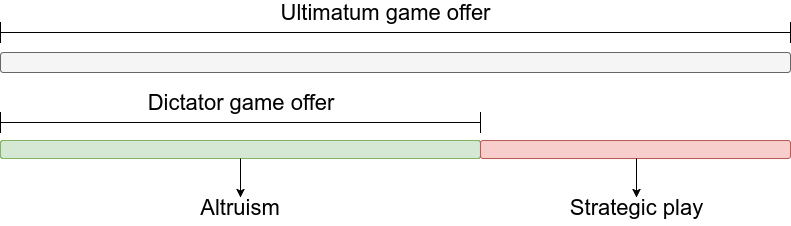
\includegraphics[width=0.8\textwidth]{dictatoroffer.png}
	\caption{Distribution of percentages sent by investors (left) and responders (right). Source: [JOHNSON 2011]}
	\label{fig:dictatorcomponent}
\end{figure}

[LEVITT AND LIST 2007] push back against the standard interpretation that positive offers in the dictator game reflect altruism and/or inequity aversion from the part of the proposer. For example, lower offers are seen when anonymity between proposer and responder is added, indicating that a concern about how one is seen by their peers is the driving force for positive offers in the dictator game. [LIST ET AL 2004] also find that, in the public goods game, the more anonymous decisions were amongst subjects the less number of subjects opted to give in the one-shot version of the game. 

[DANA ET AL 2006]  consider a variant of the dictator game where the proposer is given an initial endowment of \$10 and, after having made their choice, are offered the option of exiting the game with \$9 game. The exit option leaves the receiver nothing, but ensures that he never knows that the game has been played. Even though proposers could get a higher payoff by engaging the receiver in a dictator game and not offering anything, 28\% of the proposers opted for the exit option, perhaps because they didn't want to appear unfair to the receiver where they to enter the dictator game. In their second experiment the receiver never knows whether the money offered to them comes from the proposer or from the experimenters, thus allowing the authors to determine with more clarity whether appearing to be fair is indeed a concern for proposers. They find that 9 out of 24 proposes exited, which does imply a significant minority of proposers is concerned about not appearing self-regarding to the receivers.

In [DANA ET AL 2007] another variant of the dictator game is offered. Proposers are sorted into two different treatments, the baseline and the hidden payoff treatment. In the baseline treatment, the proposer can choose one of two actions, A and B, with respective payoffs $\left(6,1\right)$ and $\left(5,5\right)$ for the proposer and receiver respectively. In the hidden payoff treatment, the payoff for the receiver is uncertain, so proposers must choose between actions A and B where the payoffs are shown to them to be $\left(6,?\right)$ and $\left(5,?\right)$. All subjects are told that the payoffs from A and B are equally likely to be either $\left(i\right)\left(6,1\right)$ and $\left(5,5\right)$, or $ \left(ii\right)\left(6,5\right)$ and $\left(5,1\right)$. The proposer can, costlessly, choose to reveal the payoffs by clicking a button on the computer screen, and the responder is not made aware of that this choice has been made.

The prediction is that if altruism is a better motivator for the proposer's actions, he will choose B in $\left(ii\right)$ and A in $\left(ii\right)$. If instead inequity aversion is the dominant motivation, then the proportion of proposers who sacrifice one payoff unit in the baseline treatment will be the same as the proportion of proposers who click to reveal the payoffs in the hidden payoff treatment. 

14 out of 19, 74\%, of proposers in the baseline baseline treatment chose the more generous option. However, in the hidden payoff treatment, 56\% did not choose to click the button to reveal the payoffs, a difference in proportion that is statistically significant. Thus, the authors conclude that the appearance of being fair is an important determinant in dictator games and that inequity aversion does not explain the results here seen. It is possible then that at least part of the positive offers in dictator games are not because proposers are \textit{altruists} but because they are \textit{reluctant altruists}. They appear to be altruists to everyone else, but deep down they would much rather not be.



[CONCLUSAO?]

\subsection{Gift exchange and trust games}
\subsubsection{The gift exchange game}

The gift exchange game was introduced by [FEHR ET AL 1993] in an attempt to empirically investigate whether notion of fairness held by agents impeded the formation of a market clearing equilibrium in labor markets, a topic first broached in [AKERLOF 1982]. 

In the \textit{gift exchange game}, two players are each assigned one of two roles: a firm or a worker. The firm offers a wage $w$ to the worker, which the worker can then reject, in which case they both earn nothing, or accept, in which case the worker must now expend an effort level, $e$, of his choice. 

The standard prediction in such a setting can be discerned using a neoclassical model. Let's suppose the firm decides to offer the same wage to all its workers, $\omega = \bar{\omega}$. The workers have a utility function, $u(\omega,e)$, where $\omega$ is the wage rate and $e$ is the effort level they provide. The firm dictates that workers provide a minimum effort level in exchange for their wage, $e_{min}$. Workers, mindful of the firm's work rules, should choose their effort such that it maximizes:

\begin{equation}
u(\omega,e)
\end{equation}

subject to the constraints

\begin{equation}
\omega = \bar{\omega}
\end{equation}

and


\begin{equation}
e \geq e_{min}
\end{equation}


This trivial maximization problem yields the prediction that workers will choose the lowest effort level possible, $e_{min}$. The firm, aware of this, will set $\bar{\omega}$ as low as possible, in an effort to maximize profits. 

In his paper, George Akerlof [AKERLOF 1982] is motivated to explore the effects of fairness in the formation of involuntary unemployment because of the curious results coming from a study of social relations among workers at a utility company in the eastern United States [GEORGE HORMANS 1953 1954]. 

In this study, a group of women were found to be exceeding the minimum work requirements set by the firm by a considerable margin, a behavior that the neoclassical model above cannot explain. Akerlof envisions this seemingly perplexing behavior as the result of the firm and the works modelling their relationship as a "gift" exchange mediated by endogenous social norms. The workers offer a "gift" to the firm in the form of additional effort level, and in exchange the firm offers a "gift" in the form of a wage that the workers consider fair and that is in excess of what they could receive were they to leave their jobs. Thus, a labor market equilibrium is created where workers work harder because they're paid above opportunity cost, a wage level that is higher than the market clearing one, which ensures equilibrium unemployment is present. 

The gift exchange game permits us to study the level \textit{intrinsic reciprocity} in social relations such as the one described above. This reciprocity is a kind of other-regarding preference. 

Consider the following experiment from [FEHR ET AL 1997]: Subjects were assigned into one of two roles: a principal or an agent. Identities were kept anonymous, so no reputation building was possible. Principals can make a job offer to the group of agents, thus principles stand in for employers, and agents for workers.  Workers are given the option to accept or reject the offer, and, in an effort to spur competition, there are more workers than employers. The job offer consists of an incomplete contract, $\left ( w_b,e_n \right)$, that specifies a \textit{binding} wage level, $w_b$, and a \textit{non-binding} effort level, $e_n$. The choice of the effort level is represented by the choice of a number in which the higher it is the higher the effort represented is, and the higher are the monetary costs borne by the worker. As expected, the higher $e$ is the higher the payoff for the employer will be. Nothing in the experiment impedes workers from choosing an effort level that is lower than the proposed effort level in the contract, as there is no punishment for doing so. 

The expected behavior for both workers and firms are as noted earlier, that is, workers will choose the lowest possible effort level and firms, knowing this, will offer the lowest possible wage level. However, if the employer believes there are sufficiently many reciprocal workers, he has an incentive to offer higher wages in an attempt to induce higher effort levels in reciprocity. Additionally, workers may induce reciprocity by the firms by offering a higher effort level than the one initially proposed [MULTI ROUNDS?].
\\

[INSERT FIGURE]



The experimental results are depicted in [CITE FIGURE]. Two conclusions follow:

\begin{enumerate}

\item Higher desired effort levels are associated with more generous offers to the works, which suggests employers try to elicit reciprocal responses form the workers
\item \textit{On average}, the workers respond reciprocally to the employer's higher offers, though there is always a certain amount of shirking present.

\end{enumerate}

The authors further add: \textit{"there is also a substantial fraction of selfish workers who always choose the minimal effort or who rarely respond in a reciprocal manner."} The authors summarize the evidence from multiple studies to suggest that the fraction of self-regarding agents lies between 40\% to 60\%.


There remains the issue of whether laboratory findings on the impact of fairness on performance in labor market relations can be said do be externally valid.  [GNEEZY AND LIST 2006] hired students to a data-entry job where they would enter books into a library information system. Each student performed the task alone, and were offered \$12 for the job. In the experimental treatment, after the training phase, a portion of the students were informed they would receive \$20 per hour, with no explanation for the increase in pay. The control condition were payed the agreed \$12. 

The results seemed to cast doubt over the idea that offering a wage premium is an effective measure to elicit higher worker performance. In the first 90 minutes, those workers in the treatment condition produced around 25\% more than their control peers. Although this percentage difference in effort is noteworthy, the increase in effort vanished as experiment continued running and effort levels for both treatment and control conditions where found to not be significantly different. The authors interpret their results as showing that while higher wages are reciprocated by greater effort on the part of the workers, this higher effort is not persistent and thus we need be careful to extrapolate from the single round interactions in the gift exchange game to the wider world. 

A problem with [GNEEZY and LIST 2006] is that of a small sample size, which effectively limits their ability to detect statistical significance if the effect of a wage premium on effort is modest or small, a point put forward in [FEHR 2009]. Indeed, [COHN 2008] use a larger sample size and thus have enough power to detect a statistically significant increase in effort from the increased wage, thus not replicating [GNEEZY AND LIST 2006]. [FEHR 2009] surveys the literature and concludes the positive relationship between wage and effort to be robust and well replicated. 



\subsubsection{The trust game}


The \textit{trust game} is played between an \textit{investor} and a \textit{responder}. Each player is endowed with a fixed amount of tokens, $x$. The investor must decide an amount $i \leq x$ to send, or invest, to the responder, via an experimenter. The experimenter multiplies the amount sent by a multiplier $m$, meant to capture market return, and passes it on to the responder. The responder must then return an amount $r \leq mi$ back to the investor. 

If both subjects in the experiments have self-regarding preferences, then the responder will never send any money back to the investor. The investor, correctly anticipating the responder's behavior, decides to not invest any amount $i$.
\\

\begin{figure}[H]
    \centering
    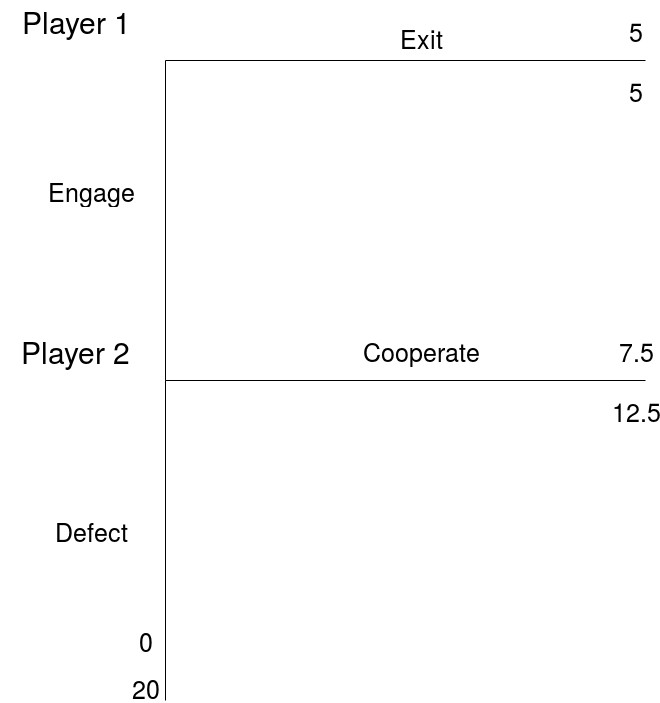
\includegraphics[width=0.6\textwidth]{trustgame.png}
    \caption{Distribution of percentages sent by investors (left) and responders (right). Source: [JOHNSON 2011]}
    \label{fig:trustgame}
\end{figure}

We can use a concrete example to prove this prediction. Let us assume a game with two players, Player 1 and Player 2. Both are each endowed with \$5. Player 1 can decide between keeping her endowment, in which case the game is ended and both players walk off with a payoff of \$5, or she may pass the entire endowment to Player 2. If the latter, the endowment is tripled by the the experimenter and Player 2 must then decide whether to keep the additional \$15 for himself, or return \$7.5 to Player 1. The payoffs are, respectively, $\left( \$ 0, \$20 \right)$, and  $\left( \$ 7.5, \$12.5 \right)$


The subgame perfect Nash Equilibrium of the trust game for the self-regarding preferences model can be determined using backwards induction. In the second stage of the game, Player 2 maximizes his payoff by defecting and walking off with the full amount. Predicting this, Player 1 will not send her endowment to Player 2. Thus, the payoff will be $\left (\$5,\$5 \right)$, i.e., both walk out with their initial endowment, having not cooperated. Traditionally, trust game experimenters allow for both players to choose how much they intend to send to the other player, but this does not change what the subgame perfect equilibrium is. 

The amount the investor is said to capture trust, and the amount sent by the responder, thrustworthiness, both forms of other-regarding preferences.

If players have self-regarding preferences, then the subgame perfect equilibrium will be met. If they have other-regarding preferences, then we should see a positive amount sent by the investor, $i>0$, and a positive amount returned by the responder, $r>0$. Figure \ref{fig:turst1} shows the distribution offers made by both investor and responder in a meta-analysis of 161 studies involving approximately 24,000 participants [CITE JOHNSON 2011].
\\



\begin{figure}[h]
    \centering
    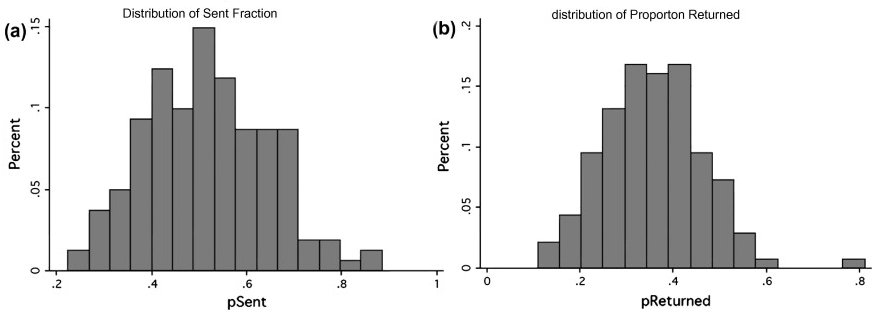
\includegraphics[width=1\textwidth]{figure_trust1.png}
    \caption{Distribution of percentages sent by investors (left) and responders (right). Source: [JOHNSON 2011]}
    \label{fig:turst1}
\end{figure}


In the meta-analysis, the mean offer made across all studies by the investor is .502, around half of the initial endowment, while the mean amount returned by the responder is .372. Due to aggregation of multiple experiments from multiple parts of the world, the authors were able to study the intercontinental differences present in the playing of the trust game, meaning, they were able to discern possible differences in levels of thrust and thrustworthiness that around the world.  They find Africa sends and receives the lowest amount of all continents, with North America and Europe leading the charge. They find further that older people send larger amounts, students send significantly lower amounts than non-students, and that amounts sent are larger if the subject believes he is playing with another human player. The evidence thus points overwhelmingly for the existence of other-regarding preferences in the trust game.
\subsection{Public goods games}
\subsubsection{Public goods game without punishments}


Let's assume a game with $n > 2$ players, each with an initial endowment of $y$ monetary units. Each player must simultaneously decide on their respective contributions, $g_i \geq 0$ to a public good. The total monetary contribution to the public good is given by $G = \sum^n_{i=1} g_i$. The monetary payoff of each individual is given by:

\begin{equation}\label{publicgoods}
    m_i = y-g_i +rG; \frac{1}{n}<r<1
\end{equation}

where $r$ is meant to represent the return, or benefit, to an individual from one unit of the public good, i.e., we can define $r$ as the marginal per capita return (MPCR).

If all players in the game have self-regarding preferences all their actions will involve \textit{free riding}, i.e, $g_i^* = 0$. To see that this is so let the vector of the contributions made by other players be $\pmb{g}_{-i}^* = \pmb{0}$. Using \eqref{publicgoods}, we see that 

\begin{equation}
\frac{\partial m_i}{\partial g_i} = r - 1 < 0
\end{equation}

which implies that the that the individual will be worse off by contributing to the public good, hence the optimal contribution is $g_i^* = 0$.

To see that the social optimum is characterized by all players contributing their full endowment $y$, note that, we can find the social optimum by solving 

\begin{equation}
\frac{\partial \sum m_i}{\partial g_i} = \frac{\partial \left( ny-G+rnG\right)}{\partial g_i} = rn-1>0 
\end{equation}

which implies that the total monetary payoff is maximized when players contribute as much as they possibly can, which in the context of this game is their full endowment $y$.

\subsubsection{Public goods game with punishments}

There's two stages to the public goods game with punishments. In the first stage the players play the public goods game without punishments. In the second stage, after the individual contributions to the public good are made publicly available, each player chooses a punishment vector $\bm{p}_i = \left( p_{i1},...,p_{in}\right)$ where $p_{ij}$ is the punishment inflicted by player $i$ on player $j$ at a cost of $c$ per unit of punishment and $0<c<1$. 

As with the game without punishments, the equilibrium for individuals with self-regarding preferences is one where all players free-ride. To see this, lets assume a vector of contributions made by$n$ players in the first round $\left(g_1,g_2,...,g_n\right)$. Independently of the vector of punishments from other players, $\pmb{p_{-i}}$, the payoff of player $i$ is maximized when $\pmb{p}_i = \pmb{0}$. Hence, it is a dominant strategy for each player not to engage in any sort of punishment, which reduces the game to the public goods game without punishments where, as saw, the Nash Equilibrium was free-riding by all players.

\subsubsection{Empirical evidence}

The evidence from one shot public goods games without punishments show little support to the idea that agents have self-regarding preferences and thus play according to the predicted equilibrium [CITE DAWES THALER 1988]. While not every subject contributes to the public good, on average, those that do contribute about 40 to 60\% of their endowment. This result does not depend on whether subjects have played the game before, on the size of the group playing, or the stakes in the game, though average contributions do lower when stakes are higher [CITE MARWELL AMES 1981)].

This general line of results is however put into question when subjects play a public goods games without punishments multiple times. What is usually seen in these cases is that in the first round the results are in line with what is observed in the one shot version of the game. However, in the following rounds, cooperation drops sharply and towards the last round the contributions for most subjects are close to zero, as predicted by the model with self-regarding preferences. [FEHR SMIDTH 1999] summarize the results from multiple repeated public goods games without punishments and say that approximately 73\% of all subjects choose to free-ride, with a significant portion of the remaining ones playing very close to the equilibrium strategy. They add that, in light of these facts, "it seems fair to say that the standard model 'approximates' the choices of a big majority of subjects rather well."

A very different picture emerges when we consider the public goods game with punishments. As we've seen, the equilibrium strategy in this version of the game is the same as in the one without punishments. Subjects are expected to free ride. However, when the possibility of punishing other players is put into the design of the experiment, close to 83\% of players choose to cooperate \textit{fully}. That is, when punishments are added, a majority of the players contribute their whole endowment towards the public good [FEHR GACHTER 2000]
\\

[FIGURE]
\\





\newpage
\section{Experimental Validity}

\newpage

\section{Moddeling Other-Regarding Preferences}

\newpage

\section{Altruism in human behavior}

A question that rises naturally from this discussion is why agents don't behave according to the game theoretic predictions when by doing so they would be better off. An argument put forward as to why agents should behave in that way is that, in a population where a percentage of the agents that follow their self-regarding preferences and another that doesn't, those that do are in an advantage. So, as time passes, those that follow their self-regarding preferences, given their increased fitness, would, through natural selection, thrive.

\newpage
\section{Conclusion}

\medskip
 
\bibliographystyle{apalike}
\bibliography{references}


\newpage
\section{Appendix}
\end{document}

\message{ !name(tese.tex) !offset(-267) }
